% Denne fil er inkluderet i udtraekning_af_regioner.tex
{
Begrebet kantdetektion dækker over en metode som finder kanterne af
objekter i et billede. Egentlig prøver man at finde de punkter i
billedet, hvor kontrasten er stor, hvilket er tilfældet ved et objekts
grænse. Når vi har fundet kanterne til objekterne i billedet kan vi
bruge disse til at afgøre hvor vi har en ny region i billedet.  Som vi
skal se, så er kantdetektion et godt eksempel på hvor svært datamatsyn
kan være, selv i meget simple algoritmer.

\subsubsection*{Metode}
Der er forskellige algoritmer til rådighed for at finde kanter i
billeder\cite{SIOlsen}. Vi vil beskrive en meget naiv tilgang til
problemet, blot for at forklare grundprincipperne bag metoden. Som
allerede nævnt vil vi finde de steder i billedet hvor vi har stor
kontrast. Det er derfor almindeligt at konvertere billedet til sort/hvid
når man vil finde kanterne. Metoden forklares for én dimension, da det
let kan overføres til to dimensioner. Vi betragter derfor en vektor
$\mathbf{P} = (p_1, p_2, \cdots, p_n)$ som antager værdier i mængden
$\{0,1\}$.

\begin{figure}[!h]
    \renewcommand{\arraystretch}{1.3}
    \centering
    \begin{tabular}{|c|c|c|c|c|c|c|c|c|c|}
        \hline
        1 & 1 & 1 & 1 & 1 & \cellcolor{black}\textcolor{white}{0} & \cellcolor{black}\textcolor{white}{0} & \cellcolor{black}\textcolor{white}{0} & \cellcolor{black}\textcolor{white}{0} & 1\\\hline
    \end{tabular}
    \caption[]{Vektoren $\mathbf{P}$ med tilfældige værdier i mængden
    $\{0,1\}$.}
    \label{vektor_p_edge}
\end{figure}
Vektoren $\mathbf{P}$ kan betragtes som et liniestykke. Vi ønsker nu at
konstruere en ny vektor $\mathbf{E} = (e_1, e_2, \cdots, e_n)$, hvor
$e_i \in \{0,1\}$ ud fra vektoren $\mathbf{P}$. Vi definerer
$\mathbf{E}$ som
\begin{equation}
    \begin{split}
        \mathbf{E} &= (e_1, e_2, \cdots, e_n) \mathrm{~,~hvor~} \\
        &e_i = \left\{
        \begin{array}{rl}
            0 & \text{hvis~} |p_i - p_{i - 1}| = 1\\
            1 & \text{hvis~} |p_i - p_{i - 1}| = 0
        \end{array} \right. \mathrm{,~for~} p_i \mathrm{~i~} \mathbf{P}
        \mathrm{~og~} p_0 = p_1
    \end{split}
    \label{vektor_e_bin}
\end{equation}
Vektoren $\mathbf{E}$ konstrueres altså ved at sammenligne et givet
punkts værdi med det forrige punkts værdi. Hvis den absolutte forskel
til et punkts forgænger er lig $1$ så sættes dette punkt til værdien $0$
i kantvektoren $\mathbf{E}$. Hvis der ikke er nogen forskel sættes værdien til
$1$. Vi er i denne sammenhæng nødt til at definere $p_0$ til $p_1$, så
vi undgår at finde en kant i starten af en linie. Kantvektoren
$\mathbf{E}$ for $\mathbf{P}$ er vist i figur \ref{vektor_e_edge}.

\begin{figure}[!h]
    \renewcommand{\arraystretch}{1.3}
    \centering
    \begin{tabular}{|c|c|c|c|c|c|c|c|c|c|}
        \hline
        1 & 1 & 1 & 1 & 1 & \cellcolor{black}\textcolor{white}{0} & 1 &
        1 & 1 & \cellcolor{black}\textcolor{white}{0} \\\hline
    \end{tabular}
    \caption[]{Kantvektoren $\mathbf{E}$ for $\mathbf{P}$.}
    \label{vektor_e_edge}
\end{figure}
Det ses at $e_6 = e_{10} = 0$, da $|p_6 - p_5| = |p_{10} - p_9| = 1$. Vi
har nu markeret de steder hvor der er kontrast i den oprindelige vektor
$\mathbf{P}$. Vi gør os en vigtig observation vedrørende definitionen på
$\mathbf{E}$. Vi markerer en kant i det punkt hvor kontrasten netop
\emph{er} skiftet. Derfor har vi også at $e_{10}$ bliver markeret som en
kant, selvom man ved manuel inspektion ville markere $e_9$ som kanten.
Dette skyldes at vi ikke har nogen hukommelse i definitionen og derfor
ikke er klar over hvilke punkter der burde hænge sammen. Vi ved altså
ikke hvilke værdier der er de interessante. Denne problematik
understreges af det faktum, at end ikke mennesket altid kan afgøre hvor
grænsen mellem to figurer går. Et klassisk eksempel er den optiske
illusion ved \emph{Rubins vase}\cite{WikiRubinVase} vist i figur
\ref{rubins_vase}. Alt efter hvad man vælger som fokus i billedet, vil
kanten skulle redefineres.

\begin{figure}[!h]
    \begin{center}
        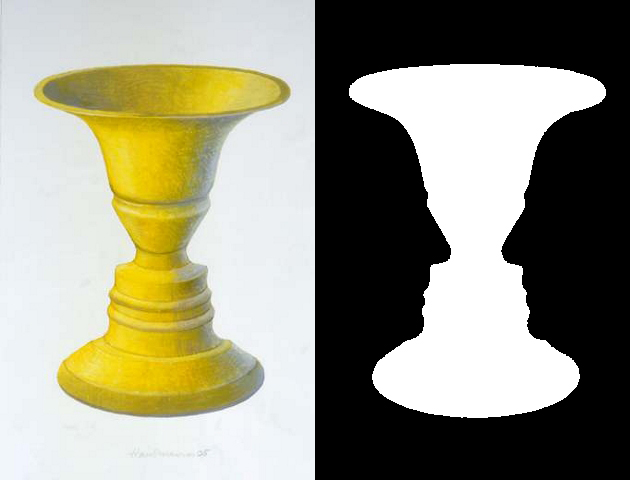
\includegraphics[trim = 84mm 4mm 0mm 0mm, clip, width=3cm]{afsnit/vores_implementation/billeder/kantdetektion/Rubin2}
    \end{center}
    \caption[]{Rubins vase\cite{WikiRubinVasePic}.}
    \label{rubins_vase}
\end{figure}

Vi kan generalisere definitionen for kantvektoren $\mathbf{E}$ i
\ref{vektor_e_bin} således at vi kan have andre værdier end dem i
$\{0,1\}$ og en anden tærskelværdi. I den følgende definition har vi at
$t$ angiver den tærskelværdi, for hvor meget værdierne punkterne imellem
må afvige.
\begin{equation}
    \begin{split}
        \mathbf{E} &= (e_1, e_2, \cdots, e_n) \mathrm{~,~hvor~} \\
        &e_i = \left\{
        \begin{array}{rl}
            0 & \text{hvis~} |p_i - p_{i - 1}| \geq t\\
            1 & \text{hvis~} |p_i - p_{i - 1}| < t
        \end{array} \right. \mathrm{,~for~} p_i \mathrm{~i~} \mathbf{P}
        \mathrm{~og~} p_0 = p_1
    \end{split}
    \label{vektor_e_generel}
\end{equation}

Definitionen på $\mathbf{E}$ tager ikke højde for støj i billedet,
hvilket let kan forvirre kantdetektionen. Sobel kantdetektion er en
etableret metode til at finde kanter i billeder. Den benytter to
foldningsmatricer til at finde kanter vertikalt og horisontalt, men er
ligesom den simple metode følsom overfor støj. Vi benytter os af en
metode udviklet af John F. Canny, da den kombinerer teknikker fra bla.
gaussisk sløring og Sobel\cite{SIOlsen}, og således ikke ligeså følsom overfor
støj. Vi vil ikke komme nærmere ind på den indre funktionalitet i Canny,
men vi vil i det følgende vise eksempler på resultater fra metoden.

\subsubsection*{Eksempler}
Vi viser nu nogle eksempler på hvordan Canny kantdetektion virker. Vi
tager igen udgangspunkt i maleriet i figur \ref{bathers}. Billedet
bliver først konverteret til gråtoner som da bruges til at finde kanter
i. Metoden returnerer et nyt sort billede med hvide kanter. Billederne
der vises er således ikke det direkte resultat fra metoden, men vi viser
kun de dele af originalbilledet hvor metoden har fundet kanter. Metoden
bruger to tærskelværdier som kan justeres alt efter hvor mange detajler
man ønsker. Vi vil ved hjælp af de følgende eksempler komme frem til
hvad tærskelværdierne betyder for resultatet. Eksemplerne er samlet i
figur \ref{canny_kanter}.

\begin{figure}[!p]
    \centering
    \subfloat[$(20, 20)$]{
        \label{canny_20_20}
        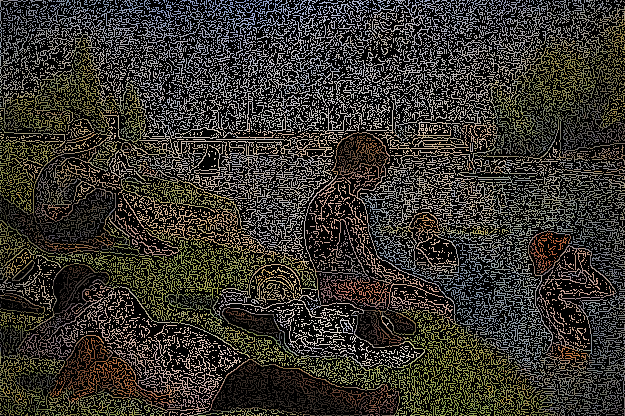
\includegraphics[width=0.6\textwidth]{afsnit/vores_implementation/billeder/kantdetektion/canny_20_20}}\\
    \subfloat[$(20, 100)$]{
        \label{canny_20_100}
        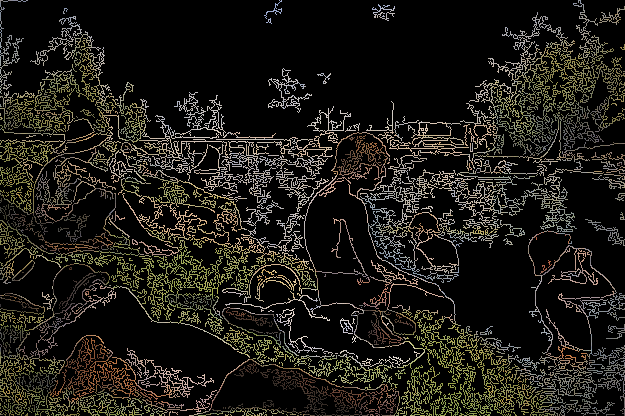
\includegraphics[angle=0,width=0.45\textwidth]{afsnit/vores_implementation/billeder/kantdetektion/canny_20_100}}\hspace{1em}
    \subfloat[$(60, 150)$]{
        \label{canny_60_150}
        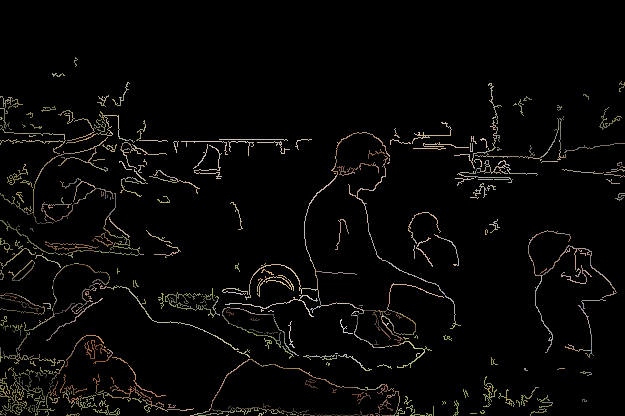
\includegraphics[angle=0,width=0.45\textwidth]{afsnit/vores_implementation/billeder/kantdetektion/canny_60_150}}\\
    \subfloat[$(70, 175)$]{
        \label{canny_70_175}
        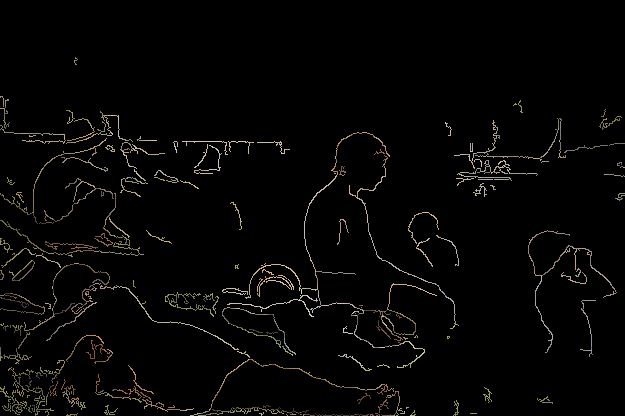
\includegraphics[angle=0,width=0.45\textwidth]{afsnit/vores_implementation/billeder/kantdetektion/canny_70_175}}\\
    \subfloat[$(100, 295)$]{
        \label{canny_100_290}
        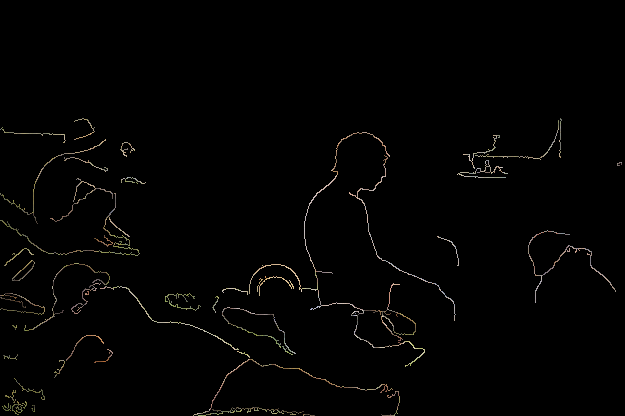
\includegraphics[angle=0,width=0.6\textwidth]{afsnit/vores_implementation/billeder/kantdetektion/canny_100_290}}
    \caption[]{Forskellige resultater med Canny kantdetektion.
    Tærskelværdierne er noteret under billederne.}
    \label{canny_kanter}
\end{figure}

Når vi sammenligner figur \ref{canny_20_20} og \ref{canny_20_100} ses
det at anden parameter lader til at ignorere kanter som ligger ``inden
for'' andre kanter. Dette ses på stort set alle personernes kroppe i
billedet. Når denne observation er gjort, prøver vi at skrue op for
tærskelværdierne. Det ses at ved højere tærskelværdier bliver billedet
med kanter gradvist mindre detaljeret. I vores testbillede er kanterne
på de fremtrædende objekter stadig at se, selv ved store tærskelværdier
som vist i \ref{canny_100_290}. Vi vil i kapitel \ref{chap_afproevning}
se på hvilke tærskelværdier vi bruger i praksis.
}

% vim: set tw=72 spell spelllang=da:
